\documentclass[twoside,11pt]{article}

\usepackage{aa222-jmlr2e}
\usepackage{amsmath}
\usepackage{graphicx}
\usepackage{listings}
\usepackage{url}
\usepackage{cleveref}
\usepackage{subcaption}
\usepackage{wrapfig}

% Compress bibliography spacing to fit 2 pages
\setlength{\bibsep}{1pt plus 0.3ex}

% Tighten vertical spacing
\setlength{\parskip}{0pt}
\setlength{\abovedisplayskip}{6pt}
\setlength{\belowdisplayskip}{6pt}

\begin{document}

\title{Final Project Proposal: Model Predictive Control for Energy-Aware Racing Line Optimization of Electric Vehicles}
\newcommand{\shorttitle}{Energy-Aware EV Racing MPC}

%===========================================
% Fill in your names and emails
%===========================================
\name{Erwin Poussi}
\email{erwinpi@stanford.edu}

\name{Matthieu Hautsch}
\email{matthaut@stanford.edu}

\maketitle

\section{Problem}
\vspace{-0.05in}

Finding the optimal racing line on a sinuous closed track is a classical problem in motorsport engineering. On straights, every driver can floor it, so there is little room for differentiation. But in corners, performance differences emerge since the racing line governs the maximum speed a car can carry through a turn, and small cornering improvements translate into significant lap time gains \citep{Xiong2010}. Beyond the geometric question of which path to follow, the vehicle dynamics (tire grip, weight transfer, drift) make this a rich nonlinear optimization problem.

We add complexity by considering electric vehicles (EVs). Unlike conventional race cars, an EV must continuously manage its battery state of charge ($SOC$). Aggressive driving drains the battery faster through increased power demand, while conservative driving preserves energy but sacrifices lap time. This creates a genuine dual-objective problem as we want to go fast \textit{and} be energy-efficient. In Formula E and the growing EV racing scene, this tradeoff directly determines race strategy.

The objective of this project is to develop an optimization-based controller that computes racing trajectories for EVs on arbitrary closed circuits, jointly minimizing lap time and energy consumption. This problem naturally decomposes into two coupled optimization stages. The first is \textbf{path optimization} (\textit{where} to drive), which seeks a racing line that exploits the full road width to reduce curvature through corners and allow higher cornering speeds. The second is \textbf{speed and control optimization} (\textit{how} to drive along that path), which determines the optimal speed profile and control inputs at every point while respecting tire grip, battery constraints, and the energy-time tradeoff. These two stages are coupled since the optimal speed depends on path curvature, and the best path depends on the vehicle's dynamic limits. Our approach addresses both through a receding-horizon formulation.

This problem fits squarely within the themes of AA222 since it involves dynamic systems modeling, nonlinear constrained optimization, and engineering design with competing objectives. It also connects to active research in eco-driving, autonomous racing, and predictive energy management \citep{Sciarretta2007, Kochenderfer2019}.

\section{Proposed Approach}
\vspace{-0.05in}

We formulate the problem as a finite-horizon \emph{Model Predictive Control} (MPC) problem. At each timestep, the controller solves an optimization over a receding horizon, applies the first control action, then re-solves with updated state information.

\vspace{-0.05in}
\subsection*{Vehicle Model}
\vspace{-0.05in}

We use a planar bicycle model capturing both longitudinal and lateral dynamics while remaining tractable. The state is $\mathbf{z} = [x,\, y,\, \psi,\, v_x,\, v_y,\, \omega,\, SOC]^\top$ (position, heading, velocities, yaw rate, battery charge) and the control inputs are $\mathbf{u} = [\delta,\, F_{\text{drive}}]^\top$, that is steering angle and net longitudinal force (positive for traction, negative for regenerative braking).

The longitudinal dynamics follow $m \dot{v}_x = F_{\text{drive}} - \tfrac{1}{2} \rho C_d A\, v_x^2 - C_r m g + m v_y \omega$, where $\rho C_d A$ captures aerodynamic drag and $C_r$ is rolling resistance. Lateral and yaw dynamics are governed by tire forces through a simplified Pacejka-like model, with the friction circle constraint $F_x^2 + F_y^2 \leq (\mu m g)^2$ ensuring we do not exceed grip.
The battery state evolves as $\dot{SOC} = -{P_{\text{elec}}}/{(Q_{\text{batt}} \cdot V_{\text{nom}})}$, where $P_{\text{elec}} = {F_{\text{drive}} \cdot v_x}/{\eta}$, with motor efficiency $\eta$ (accounting for regen when $F_{\text{drive}} < 0$), battery capacity $Q_{\text{batt}}$, and nominal voltage $V_{\text{nom}}$.

\vspace{-0.05in}
\subsection*{Optimization Formulation}
\vspace{-0.05in}

We minimize the weighted cost
\vspace{-0.05in}
\[
J = \underbrace{w_t \cdot T_{\text{lap}}}_{\text{time}} + \underbrace{w_e \cdot \Delta SOC}_{\text{energy}} + \underbrace{w_u \int_0^{T} \|\dot{\mathbf{u}}\|^2 \, dt}_{\text{smoothness}}
\]

\vspace{-0.1in}
\noindent subject to: speed bounds $\|\mathbf{v}\| \leq v_{\max}$, actuation limits $|F_{\text{drive}}| \leq F_{\max}$ and $|\delta| \leq \delta_{\max}$, battery limits $SOC_{\min} \leq SOC \leq 1$, tire grip $F_x^2 + F_y^2 \leq (\mu m g)^2$, and track boundary constraints. By varying $w_t$ and $w_e$, we explore the Pareto front between lap time and energy consumption.

\vspace{-0.05in}
\subsection*{Experimental Setup}
\vspace{-0.05in}

\begin{wrapfigure}{r}{0.42\textwidth}
    \vspace{-0.2in}
    \centering
    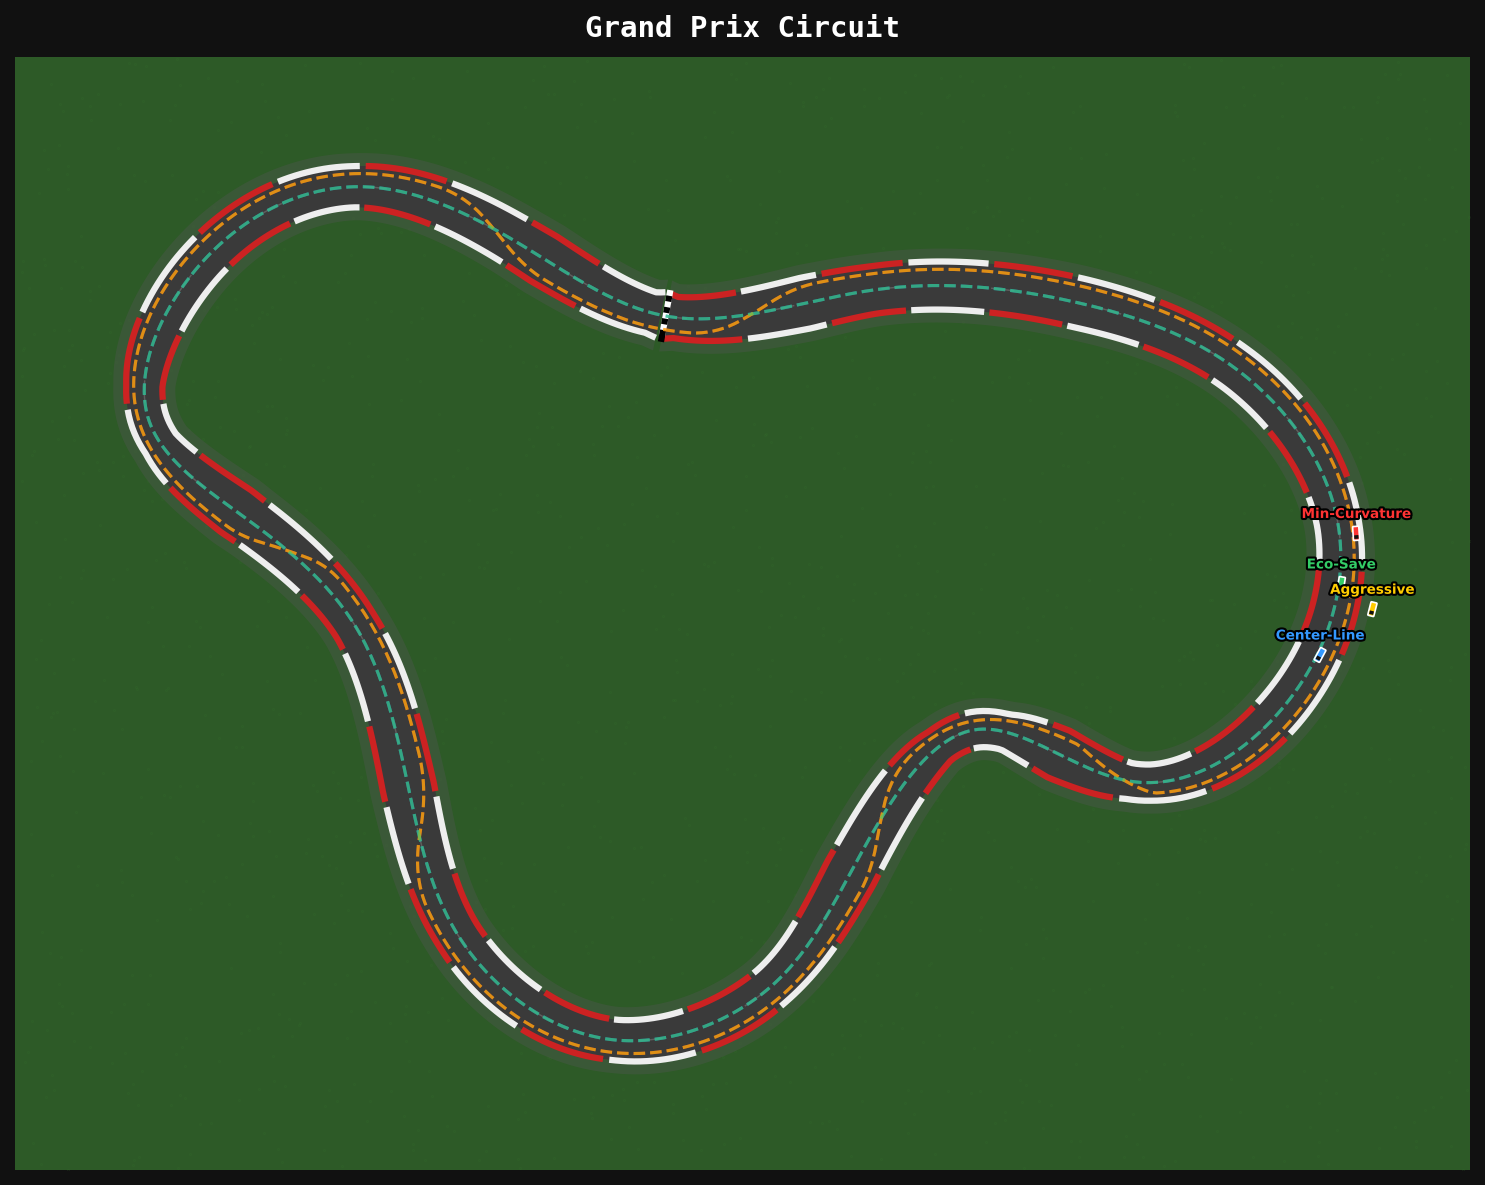
\includegraphics[width=0.40\textwidth]{../figures/track_with_raceline.png}
    \vspace{-0.1in}
    \caption{Simulated circuit with track boundaries and center-line.}
    \label{fig:track_example}
    \vspace{-0.15in}
\end{wrapfigure}

We plan to test the controller on several simulated closed circuits of varying complexity (from simple ovals to circuits with tight hairpins and chicanes), as shown in \cref{fig:track_example}.

\textbf{Baselines.}
We will benchmark against: (1)~constant-speed center-line following, (2)~minimum-time aggressive driving (ignoring energy), (3)~minimum-curvature path planning \citep{Heilmeier2020}, and (4)~a heuristic energy-saving strategy.

\textbf{Metrics.}
Performance will be evaluated on: lap time $T_{\text{lap}}$, energy consumed $\Delta SOC$, ride smoothness $\int \|\dot{\mathbf{u}}\|^2 dt$, and solver runtime. We will also construct Pareto fronts between lap time and energy use.

\enlargethispage{0.3in}
\vspace{-0.15in}
\begingroup
\small
\bibliography{references}
\endgroup

\end{document}
